% !TeX spellcheck = en_US
\documentclass[11pt, a4paper]{article}
\usepackage[utf8]{inputenc}

\usepackage{latexsym}
\usepackage{float}
\usepackage[utf8]{inputenc}
\usepackage[english]{babel}
\usepackage{microtype}
\usepackage[hyphens]{url}
\usepackage{hyperref}
\usepackage{graphicx}
\usepackage{makeidx}
\usepackage{datetime}
\usepackage{multicol}
\usepackage{setspace}
\usepackage{pdflscape}
\usepackage{pgffor}
\usepackage{enumerate}
\usepackage{booktabs}
\usepackage{tabularx}
\usepackage{braket}
\usepackage{listings}
\usepackage{color}
\usepackage{amsmath}
\usepackage{amssymb}
\usepackage[table,xcdraw]{xcolor}
\usepackage{graphicx}
\usepackage{listings}
\usepackage{hyperref}
\usepackage{vmargin}
\usepackage{wrapfig}
\usepackage{subfiles}
\usepackage{float}
\usepackage{amsmath}
\usepackage{amssymb}
\usepackage{tikz-cd}
\usepackage{multirow}
\usepackage{pgffor}
\usepackage{enumitem}
\usepackage{iflang}
\usepackage{varioref}
\usepackage{hyperref}
\usepackage{cleveref}
\usepackage{caption}
\usepackage{subcaption}
\usepackage{tikz}
\usepackage{enumitem}
\usepackage{xpatch}
\usepackage{refcount}
\usepackage{color}
\usepackage{pdfpages}
\usepackage{array}
\usepackage{eurosym}
\usepackage{longtable}

%%%%%%%%%%%%%%%%%%%%%%%%%%%%%%%%%%%%%%%
%%%%%%%%%%%% UTIL COMMANDS %%%%%%%%%%%%  

\setcounter{secnumdepth}{4}
\newcommand{\nc}{\newcommand}
\nc{\supindex}{\textsuperscript}
\renewcommand{\baselinestretch}{1.5}
\nc{\myparagraph}[1]{\paragraph{#1}\mbox{}\\}

%%%%%%%%%%%%%%%%%%%%%%%%%%%%%%%%%%%%%%%
%%%%%%%%%%%%% CONFIG FILE %%%%%%%%%%%%%

\nc{\mytitle}{Economic Viability}
\nc{\mysubtitle}{Bayesian Inference}
\nc{\authors}{
	Oriol Alàs Cercós, Sergi Simón Balcells}
\nc{\datetime}{1\supindex{st} of June, 2022}
\nc{\assignatura}{HIgh Performance Computing}
\nc{\professorat}{Jordi Ricard Onrubia Palacios}

% Per separar professors, utilitzar ','
% 	Ex: Maria, Joan, Pere

%%%%%%%%%%%%%%%%%%%%%%%%%%%%%%%%%%%%%%%
%%%%%%%%%%%%%  LANGUAGE   %%%%%%%%%%%%%

\newcommand{\tr}{\IfLanguageName{english}}

%%%%%%%%%%%%%%%%%%%%%%%%%%%%%%%%%%%%%%%
%%%%%%%%%%%%%%%%% MATH %%%%%%%%%%%%%%%%

\nc{\prob}[1]{P({#1})}
\nc{\probl}[2]{P({#1}|{#2})}

%%%%%%%%%%%%%%%%%%%%%%%%%%%%%%%%%%%%%%%
%%%%%%%%%%%%% FUNCTIONS %%%%%%%%%%%%

\nc{\numitems}[1]{\getrefnumber{#1}}
\newcounter{itemcntr}
\AtBeginEnvironment{itemize}{%
	\setcounter{itemcntr}{0}%
	\xapptocmd{\item}{\refstepcounter{itemcntr}}{}{}%
}

%%%%%%%%%%%%%%%%%%%%%%%%%%%%%%%%%%%%%%%
%%%%%%%%%%%%% RADIO BUTTON %%%%%%%%%%%%

\makeatletter
\newcommand*{\radiobutton}{%
	\@ifstar{\@radiobutton0}{\@radiobutton1}%
}
\newcommand*{\@radiobutton}[1]{%
	\begin{tikzpicture}
		\pgfmathsetlengthmacro\radius{height("X")/2}
		\draw[radius=\radius] circle;
		\ifcase#1 \fill[radius=.6*\radius] circle;\fi
	\end{tikzpicture}%
}
\makeatother


%%%%%%%%%%%%%%%%%%%%%%%%%%%%%%%%%%%%%%%
%%%%%%%%%%%%%  %%%%%%%%%%%%


\newcolumntype{S}{>{\centering\arraybackslash}m{1.5em}}

\renewcommand{\tabularxcolumn}[1]{m{#1}} % redefine 'X' to use 'm'
\newcommand{ \titem}[1]{\item \textbf{#1}\quad}

\newcommand{\costVar}[4]{In that moment, we want to earn $\frac{#1\text{€}}{1 h}$, therefore the human resource cost will be: \[#2 \cdot \frac{#3h}{1 day} \cdot \frac{#1\text{€}}{1 h} = #4 \text{€}\] }

\nc{\numbers}[1]{
	\begin{tabularx}{#1\textwidth}{|S|S|S|S|S|}
		\hline 1 & 2 & 3 & 4& 5 \\\hline
	\end{tabularx}
}

\nc{\optionsofcol}{
	\multicolumn{3}{c}
	{%
		\numbers{0.338}
	}
}

\nc{\options}{\multicolumn{2}{c}
	{%
		\numbers{0.338}
}}

\newcommand{\costHR}[4]{\[Cost_{\text{HR}} = #1 \frac{\text{€}}{h} \cdot \frac{#2 \, \, \text{hours}}{\text{day}} \cdot #3 \, \, \text{days} = #4 \, \, \text{€} \]}

\newcolumntype{P}[1]{>{\centering\arraybackslash}p{#1}}

\setpapersize{A4}

\author{Oriol Alàs Cercós}
\date{29 d'Abril del 2019}

\def\contentsname{Índex}
\begin{document}
	
	\definecolor{gray}{rgb}{0.4,0.4,0.4}
	\definecolor{darkblue}{rgb}{0.0,0.0,0.6}
	\definecolor{cyan}{rgb}{0.0,0.6,0.6}
	\lstset{
		basicstyle=\ttfamily,
		columns=fullflexible,
		showstringspaces=false,
		commentstyle=\color{gray}\upshape
	}
	
	\lstdefinelanguage{XML}
	{
		morestring=[b]",
		morestring=[s]{>}{<},
		morecomment=[s]{<?}{?>},
		stringstyle=\color{black},
		identifierstyle=\color{darkblue},
		keywordstyle=\color{cyan},
		morekeywords={xmlns,version,type}% list your attributes here
	}
	
	\begin{titlepage}
		\begin{figure}[htb]
			\begin{center}
				
				\includegraphics[width=5cm]{imgs/udl.png}\\
				
				
				\medskip
				\begin{center}
					
					\huge\textbf{\mytitle}\\
					\bigskip
					\normalsize{\tr{Made by}{Realitzat per:}}
					\\
					\large\textit{\authors}
					\\
					\setlength{\parskip}{1em}
					\normalsize{\tr{Delivery}{Data de lliurament:}}
					\\
					\large{\datetime}
				\end{center}
				
				\vspace*{\stretch{2.0}}
			\end{center}
		\end{figure}
		\begin{flushright}
			Universitat de Lleida
			\\
			Escola Politècnica Superior
			\\
			Màster en Enginyeria Informàtica
			\\
			\assignatura
			\\
			\medskip
			\textbf{\tr{Professorate:}{Tutor:}}
			\\
			\foreach \n in \professorat{\n\\}
		\end{flushright}
		\thispagestyle{empty} 
	\end{titlepage}
	\pagenumbering{roman}
	\tableofcontents
	\listoffigures
	\listoftables
	\newpage
	\pagenumbering{arabic}
	
	\section{Introduction}
	
	The project consists of developing the game of life program in a parallelized environment using MPI + OpenMP. This work is based on the MPI program, so feel free to skip the 2nd section if you have read that work. The first sections will be which parallel algorithms we could use, which one we choose, and why we did it. We will also discuss the project structure, as a single file was not readable when developing with MPI. \\
	\\
	Then, we will provide the results of this code executed at the Moore cluster with the examples of 5000 and 10000 matrices provided in the assignment. In the following section, we will analyze why the application behaves like that.\\
	\\
	Finally, a conclusion to the analysis is provided, where we remark on the key points that were discovered in it.
	\section{Algorithm Selected}
	The algorithm could take three shapes depending on which communication the nodes use:
\begin{enumerate} % TODO make square message.
	\item Divide the square into smaller squares. This solution is inefficient in terms of communication, as it has to send and receive data from 4 other cores, as seen in the figure \ref{fig:matrix}.
	%
\begin{figure}[H]
	\centering
	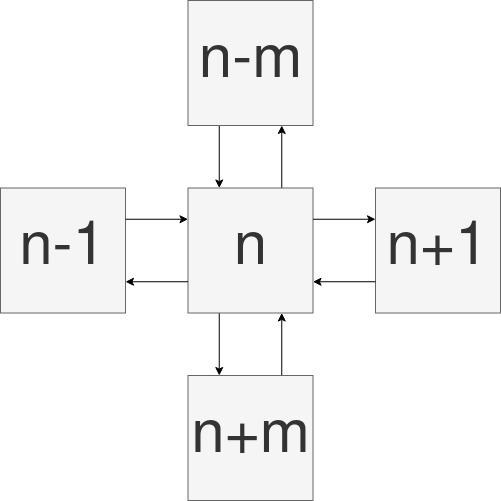
\includegraphics[width=0.4\linewidth]{imgs/matrix}
	\caption[Matrix Communication]{Matrix figure to showcase the algorithm. In this example, a node connects to all the four neighbors.}
	\label{fig:matrix}
\end{figure}
	%
	\item Divide the matrix into columns. This solution is better than before, as it only sends the information to two other nodes, making the transportation less painful.
%
\begin{figure}[H]
	\centering
	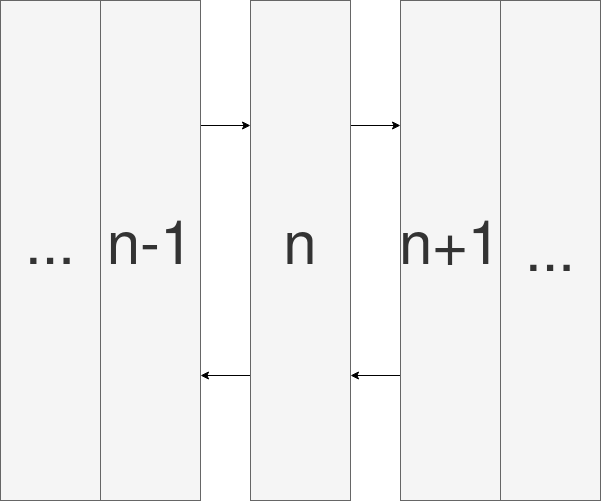
\includegraphics[width=0.4\linewidth]{imgs/rows}
	\caption[Columns Communication]{Columns figure to showcase the algorithm. In this example, a node connects to two neighbors}
	\label{fig:columns}
\end{figure}
%
	\item Divide the matrix into rows. The same as the last one, but it has better memory allocation, as the items are next to each other in the memory.
	%
\begin{figure}[H]
	\centering
	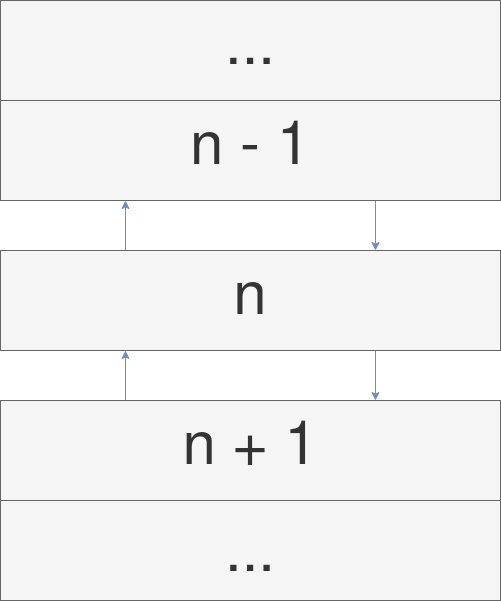
\includegraphics[width=0.4\linewidth]{imgs/columns}
	\caption[Rows Communication]{Rows figure to showcase the algorithm. In this example, a node connects to two neighbors}
	\label{fig:columns}
\end{figure}
	
\end{enumerate}

So, for said reasons, we will be developing our program with the communication orientated to rows.\\
\\
Although MPI is a relatively high-level interface, it does not provide as much abstraction as one would desire, so there is more boilerplate code to achieve the parallelization of the program. As such, the code quickly became a hassle to navigate, so it was divided into some other modules, which are:
\begin{description}
	\item[\texttt{contants.h}] This module contains all the constants that the program uses, as the debug constant. All the constants are declared as \texttt{const type} if they are not used by arrays, to avoid the VLAs.
	
	\item[\texttt{debug\_tools.h}] Inside this file some utilities only execute if the debug option is set to true. This, combined with an optimization 3 on the compiler makes all the debug functions disappear in the end code.
	
	\item[\texttt{mpi\_utilities.h}] Most of the commands to send and receive from the MPI are repeated through the code. This file contains an abstraction layer to avoid them.
	
	\item[\texttt{utilities.h}] Some functions that the professor provided us.
	
	\item[\texttt{read\_life.h}] This file contains all the functions regarding the reading or creation of the matrix to perform the game of life, as well as the necessary communication with all the nodes for their table.
	
	\item[\texttt{update\_file.h}] This module contains all the functions related to doing an update of the game of life. It also contains all the necessary communication between these modules.
	
	\item[\texttt{main.c}] Contains the executable, as well as some little functions.
\end{description} 
\vspace{0.75cm}

Finally, the compilation of this program was:
\begin{verbatim}
	mpicc -o main main.c -O4 -std=gnu99
\end{verbatim}
Where O4 activates the optimizations, it also is specified to compile the source with gnu99, as it used a non-compatible version with the code by default. Although 3 should be more than enough, in some systems it does not work as intended. 

\section{Changes from the last algorithm}
As usual, we discussed the previous solution with the companions that delivered the work. One of the optimizations we talked about was the change in the types. As at most, the support matrix can have 5, and the grid matrix can only be either ones or zeros, so using \texttt{int8\_t} instead of 64 bits integers are faster, as the cost of the network is lower. Additionally, we changed so we only allocate the support matrix once, and free it once the program finishes. Still, this was already done by the compiler, so it didn't improve the performance. As we will comment on the analysis, the performance of the program was slower than it was expected, so we tried to optimize the code more. After a time of searching, we discovered the reason for the slowness of the program, as will be discussed in the results.

	\section{Results}
				The results are gathered separated by the size used. Each of them between how many threads the OpenMP uses. The number of nodes used by the MPI is the number of slots divided by the number of threads.
			\\
			\\
	The time measured in these graphics and tables is the time that the application needs to read the file and update until the maximum number of iterations is met.
	\newcommand{\speedup}[1]{
	\caption[Speedup #1]{Speedup table. There are two examples used in this process, both being square matrixes of #1 specifically.}
	\label{tab:speedup}\\
	
}
	\newcommand{\timetable}[1]{
\caption[Time #1]{Time table. There are two examples used in this process, both being square matrixes of #1 specifically.}
\label{tab:time}\\
	
}
\newcommand{\efficiency}[1]{
	\caption[Efficiency #1]{Efficiency table. There are two examples used in this process, both being square matrixes of #1 specifically.}
\label{tab:efficiency}\\
}
	\subfile{tables/time-5000.tex}
	\subfile{tables/speedup-5000.tex}
	\subfile{tables/efficiency-5000.tex}
	
	\subfile{tables/time-10000.tex}
	\subfile{tables/speedup-10000.tex}
	\subfile{tables/efficiency-10000.tex}
	
	\newcommand{\timeplot}[1]{
				\includegraphics[width=0.7\linewidth]{plots/time-#1}
		\caption[Time Plot #1]{Time plot. The y axis is the time in seconds while the x axis is the number of cores used. This is only for the #1 sized matrix.}
		\label{fig:time-#1}
	}
	
	\newcommand{\speedupplot}[1]{
	\includegraphics[width=0.7\linewidth]{plots/speedup-#1}
	\caption[Speedup plot #1]{Speedup plot. The y axis is the speedup while the x axis is the number of cores used. This is only for #1 sized matrix}
	\label{fig:speedup-#1}
}


\newcommand{\efficiencyplot}[1]{
\includegraphics[width=0.7\linewidth]{plots/efficiency-#1}
\caption[Efficiency plot #1]{Efficiency plot. The y axis is the efficiency while the x axis is the number of cores used. This is only for #1 sized matrix}
\label{fig:efficiency}
}
	\begin{figure}[H]
		\centering
		\timeplot{5000}
	\end{figure}
	
	\begin{figure}[H]
		\centering
		\timeplot{10000}
	\end{figure}
	
	\begin{figure}[H]
		\centering
		\speedupplot{5000}
	\end{figure}
	
	
	\begin{figure}[H]
		\centering
		\speedupplot{10000}
	\end{figure}
	
	\begin{figure}[H]
		\centering
		\efficiencyplot{5000}
	\end{figure}

\begin{figure}[H]
	\centering
	\efficiencyplot{10000}
\end{figure}

	\subsection{Analysis}
	The cost analysis is the same as the previous work. As such we will divide the analysis into two sections, the formal analysis and a secondary analysis where we will analyze why OpenMP performs worse than the MPI counterpart. Feel free to skip the first section if you have already read the MPI project.
	\section{Formal Analysis}
	This application is almost embarrassingly parallel, as the costs and the speedup increase linearly with the number of cores that uses them. But, there is a small bottleneck that is reading the file: as the disc storage is not concurrent, the reading must be set to read in parallel. Furthermore, For this reason, it can be seen that the efficiency worsens in each core added, as that part of the program is sequential.\\
\\
This pattern can be seen more clearly at the efficiency plot, as the efficiency limits to the part of the code that can not be done concurrently, as shown in the next formula:
\[ \lim_{x \to \infty} E(x) = \lim_{x \to \infty} \frac{T_s} {(T_{\text{read file}} +  \frac{T_p + T_\text{communication}} x ) \cdot x} \]
\[= lim_{x \to \infty}\frac{T_s}{T_\text{read file} \cdot x + T_p + T_{\text{communication}}} = 0\]
This means that the efficiency will eventually reach 0, as the time spend reading the file, and communicating with the other two nodes will never be parallelized. This also means that the maximum speed up is:
\[ \lim_{x \to \infty} S(x) = \lim_{x \to \infty} \frac{T_s}{T_{\text{read file}} + \frac{T_p + T_\text{communication}}x} = \frac{T_s}{T_\text{read file}}\]
\\
What's more, this pattern is shockingly the same with both benchmarks that were tried, where the maximum difference in speedup is $1.18$, and both speedups are close to each other. With the median of 100 executions, this difference may be even lower. Furthermore, the efficiency also shows that the change when the overheat of communication as the number of nodes increases is maintained through all the executions, and it slowly decays as the reading of the file cannot be parallelized. 

\section{Why MPI is faster}
Hybrid computing is always faster than only using an MPI counterpart, as the communication between sockets is slower than the memory counterparts. Nevertheless, both MPI and OpenMP experts discourage using MPI + OpenMP, as \cite{openmp}, and \cite{article} says. More understandably and concisely, when using optimizations with the compiler, the overheating of using both technologies shadows the more efficient approach of using a hybrid system. This is the way MPI has included a threaded option, as well as some directives to make the hybrid approach faster, even if it is not as easy as OpenMP.\\
\\
This is concluded when comparing the 32 slots using a hybrid approach versus using only MPI, where in this project it takes 32 seconds with the hybrid, and only 16 seconds with MPI, even without the memory optimizations.
	\section{Conclusion}
	In this project we parallelized the algorithm of the Game of Life, reaching almost embarrassingly parallel levels of concurrency in the program with the correct use of the scheduler and the optimizations in the MPICC set to maximum\\
\\
Moreover, it was determined that both the reading part of the game of life and the communication part is the only sequential part of the whole operation, which makes the efficiency slow down as the number of cores rises, where eventually it will reach 0. Additionally, the speedup is theoretically relative to the sum of the time spent reading the file, as well as the time spent communicating with two nodes.\\
\\
Nevertheless, it was stated that only MPI, with the optimizations of the compiler enabled is faster than the hybrid counterpart, as the overheat of using OpenMP overshadows the communication cost of MPI. It was stated that most probably using only MPI + MPI as an hybrid solution will be faster than all the solutions.
	\bibliography{bibliography}
	\bibliographystyle{unsrt}
	
\end{document}
